% Methodology

\begin{figure}
    \centering
    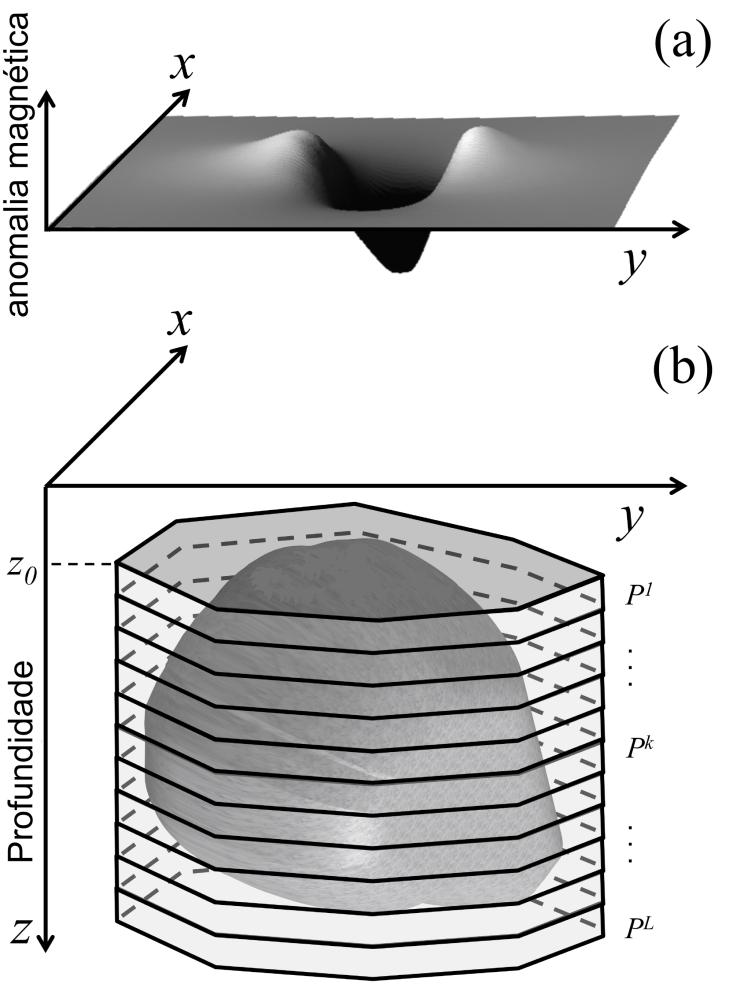
\includegraphics[scale=1]{figures/observed_data.png}
    \caption{Schematic representation of (a) total-filed anomaly (gray surface) produced by (b) a 3-D anomalous source (dark gray volume). The interpretation model in (b) consists of a set of L vertical, juxtaposed 3-D prisms $P^k$ , $k = 1,\dots, L$, (light gray prisms) in the vertical direction of a right-handed coordinate system.}
    \label{fig:obs}
\end{figure}

\begin{figure}
    \centering
    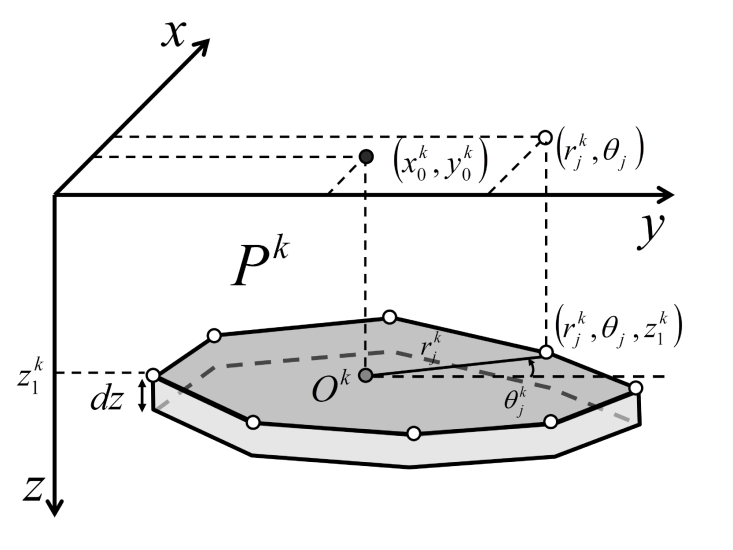
\includegraphics[scale=0.3]{figures/prism_parameters_mod.png}
    \caption{Polygonal cross-section of the $k$th vertical prism $P^k$ described by $V$ vertices (white dots) with polar coordinates ($r^k_j$ , $\theta ^k_j$), $j = 1, \dots, V$, $k = 1, \dots, L$ , referred to an arbitrary origin $O^k$ (grey dot) with horizontal Cartesian coordinates ($x_0^k$ , $y_0^k$), $k = 1, \dots, L$ , (black dot).}
    \label{fig:prism_parameters}
\end{figure}

% Application to synthetic data - simple model

\begin{figure}
    \centering
    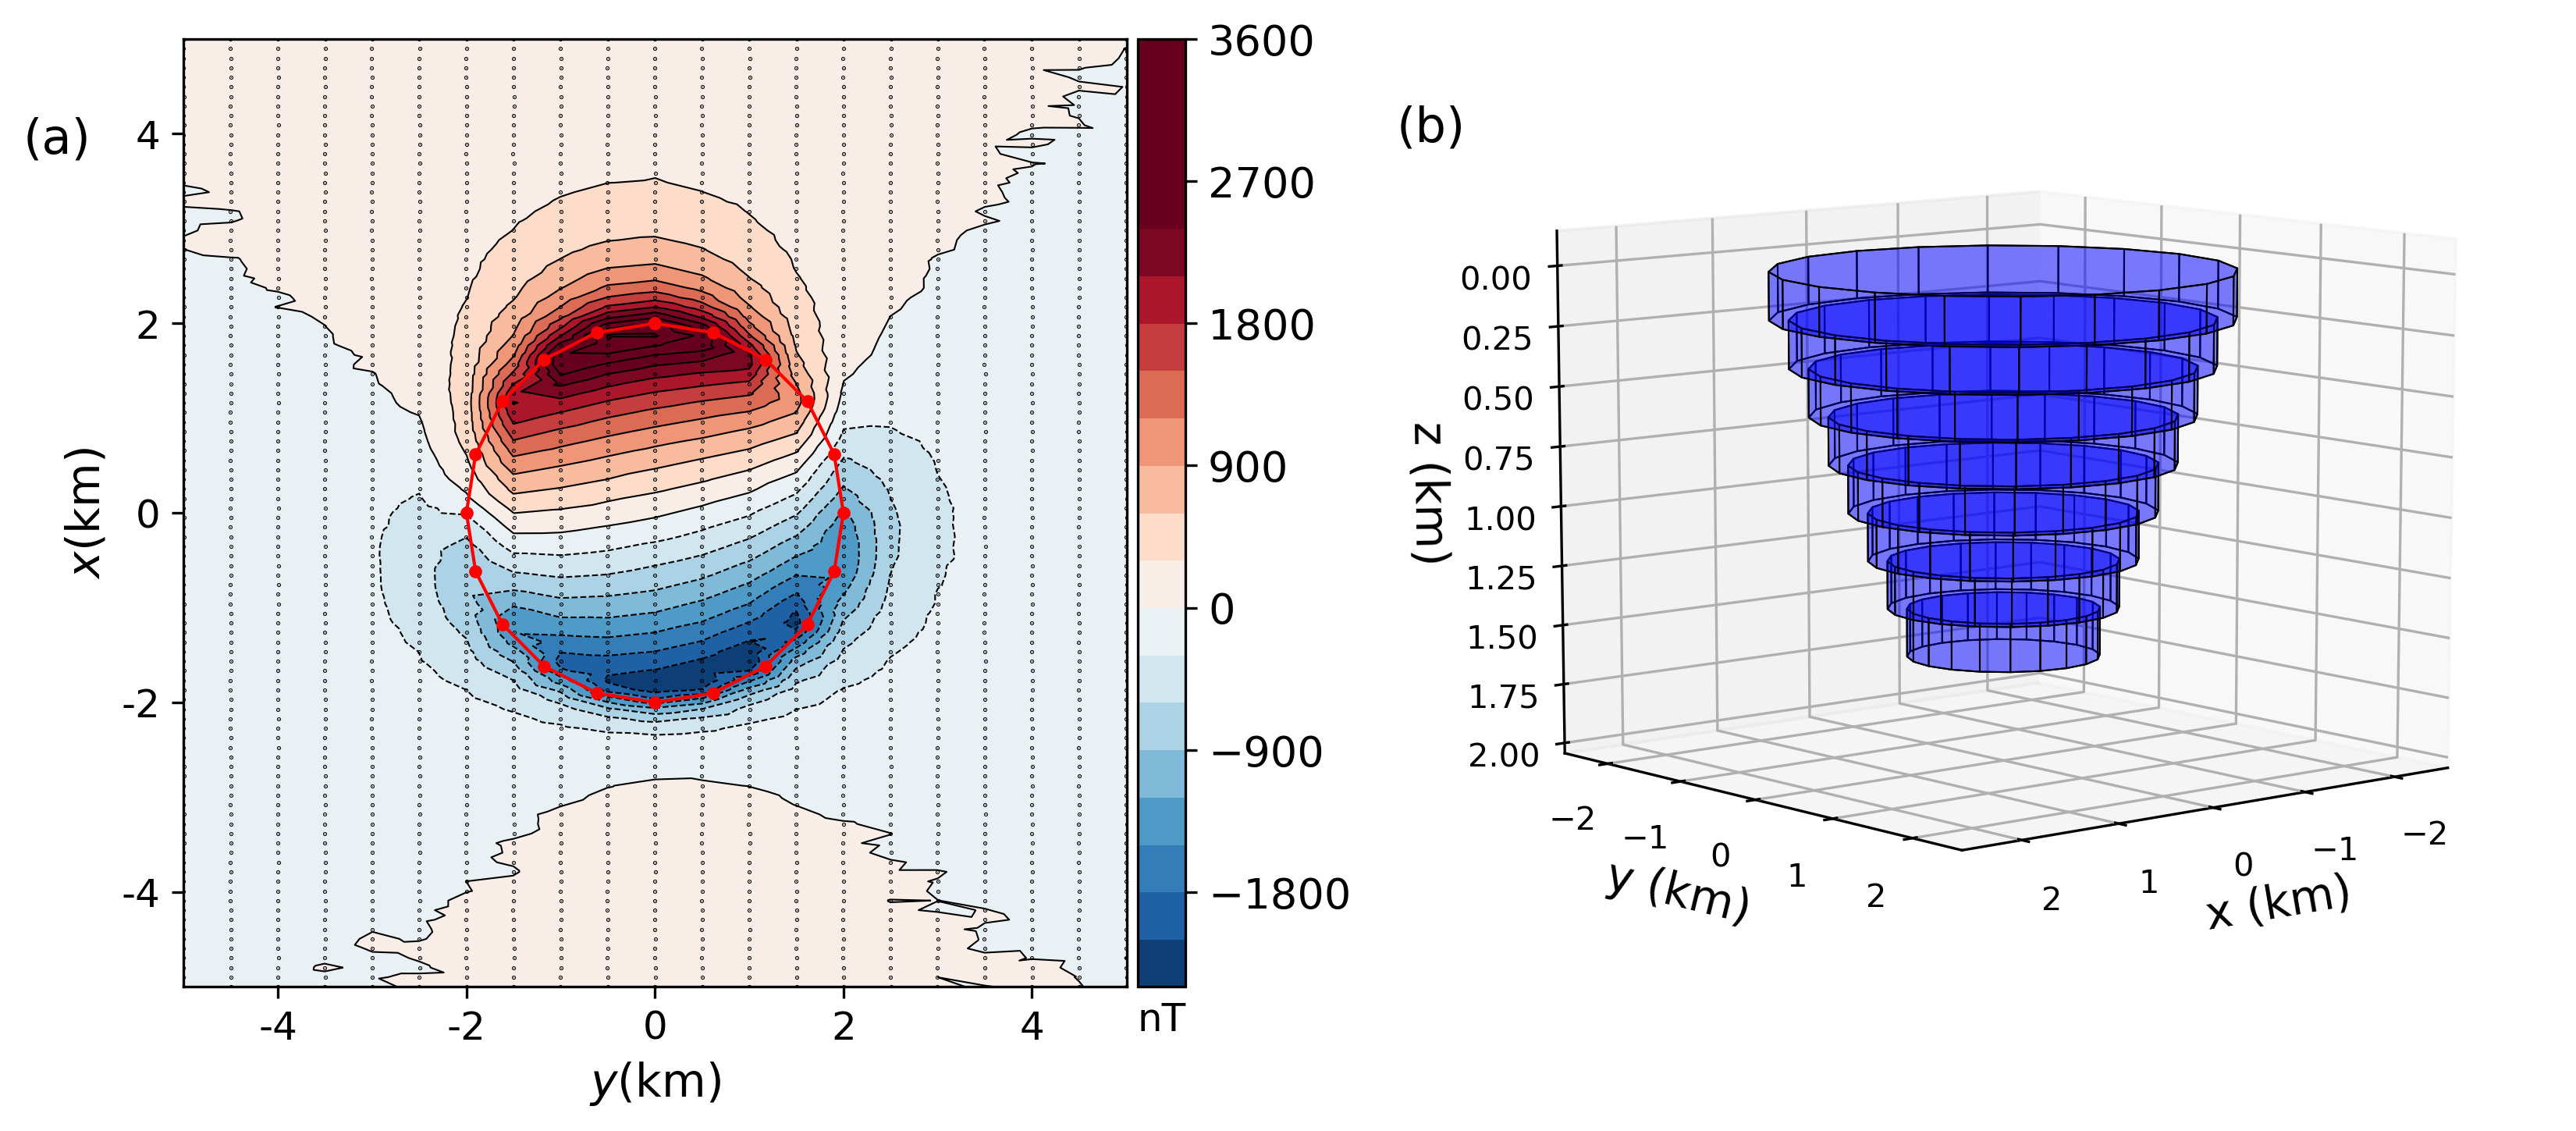
\includegraphics[scale=.5]{figures/simple_model_data.png}
    \caption{Simple model simulation. (a) Noise-corrupted total-field anomaly produced by the simple model (blue prisms) in (b) with a pseudoramdom Gaussian distribution having mean $\mu_0 = 0$ nT and standard deviation $\sigma_0 = 5$ nT, the black dots represent the observation points. The connected red dots are the vertices of the initial approximate horizontally projected at the data map. (b) Perspective view of the simple model represented by the blue prisms.
}
    \label{fig:simple_model}
\end{figure}

\begin{figure}
	\centering
	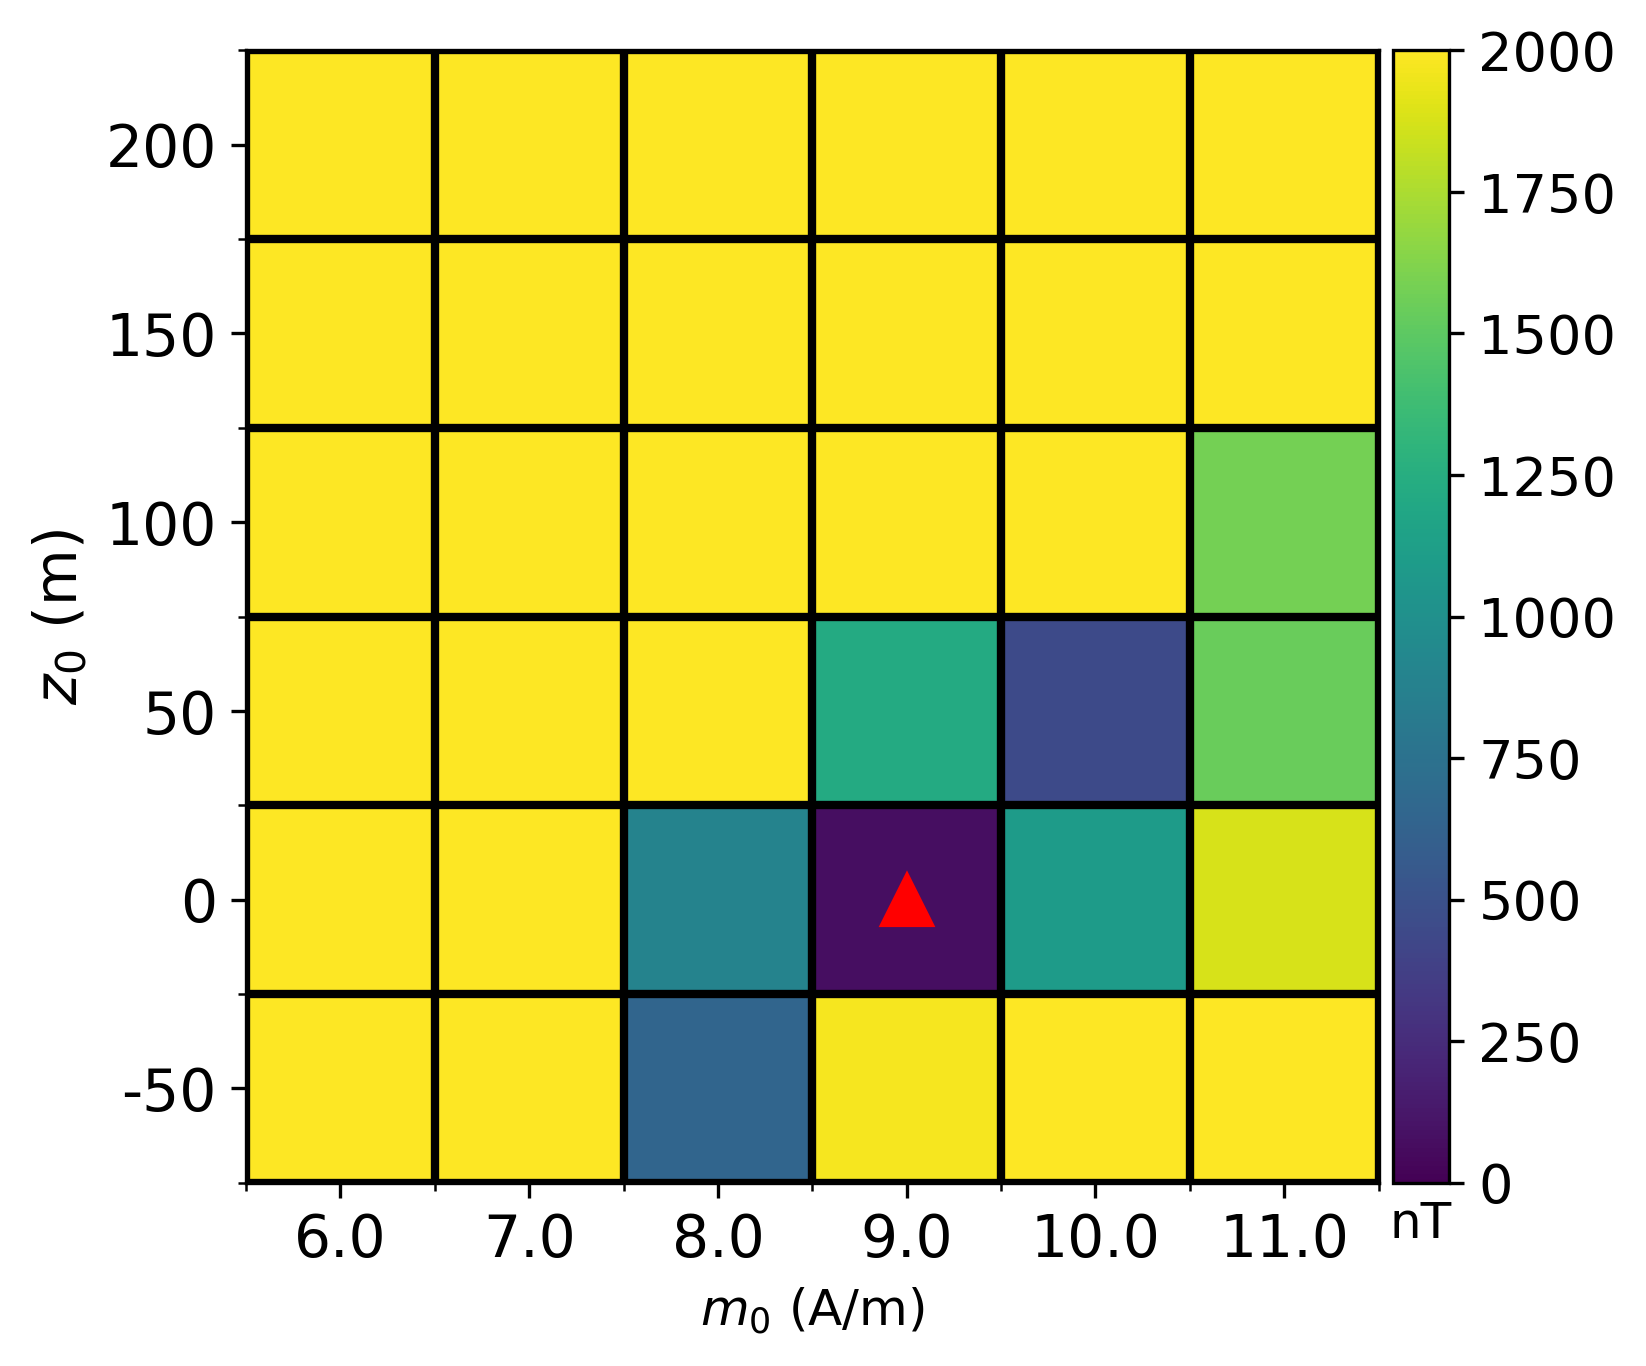
\includegraphics[scale=.75]{figures/simple_gamma.png}
	\caption{Application to the simple model data. 
	Goal function $\Gamma(\mathbf{p})$ (eq. \ref{eq:gamma}), in nT,  
	produced by estimated models with different depths-to-the-top ($ z_0 $) and 
	total-magnetization intensities ($ m_0 $). 
	The red triangle represents the $m_0$ and $z_0$ of the true source.}
	\label{fig:simple_map}
\end{figure}

\begin{figure}
	\centering
	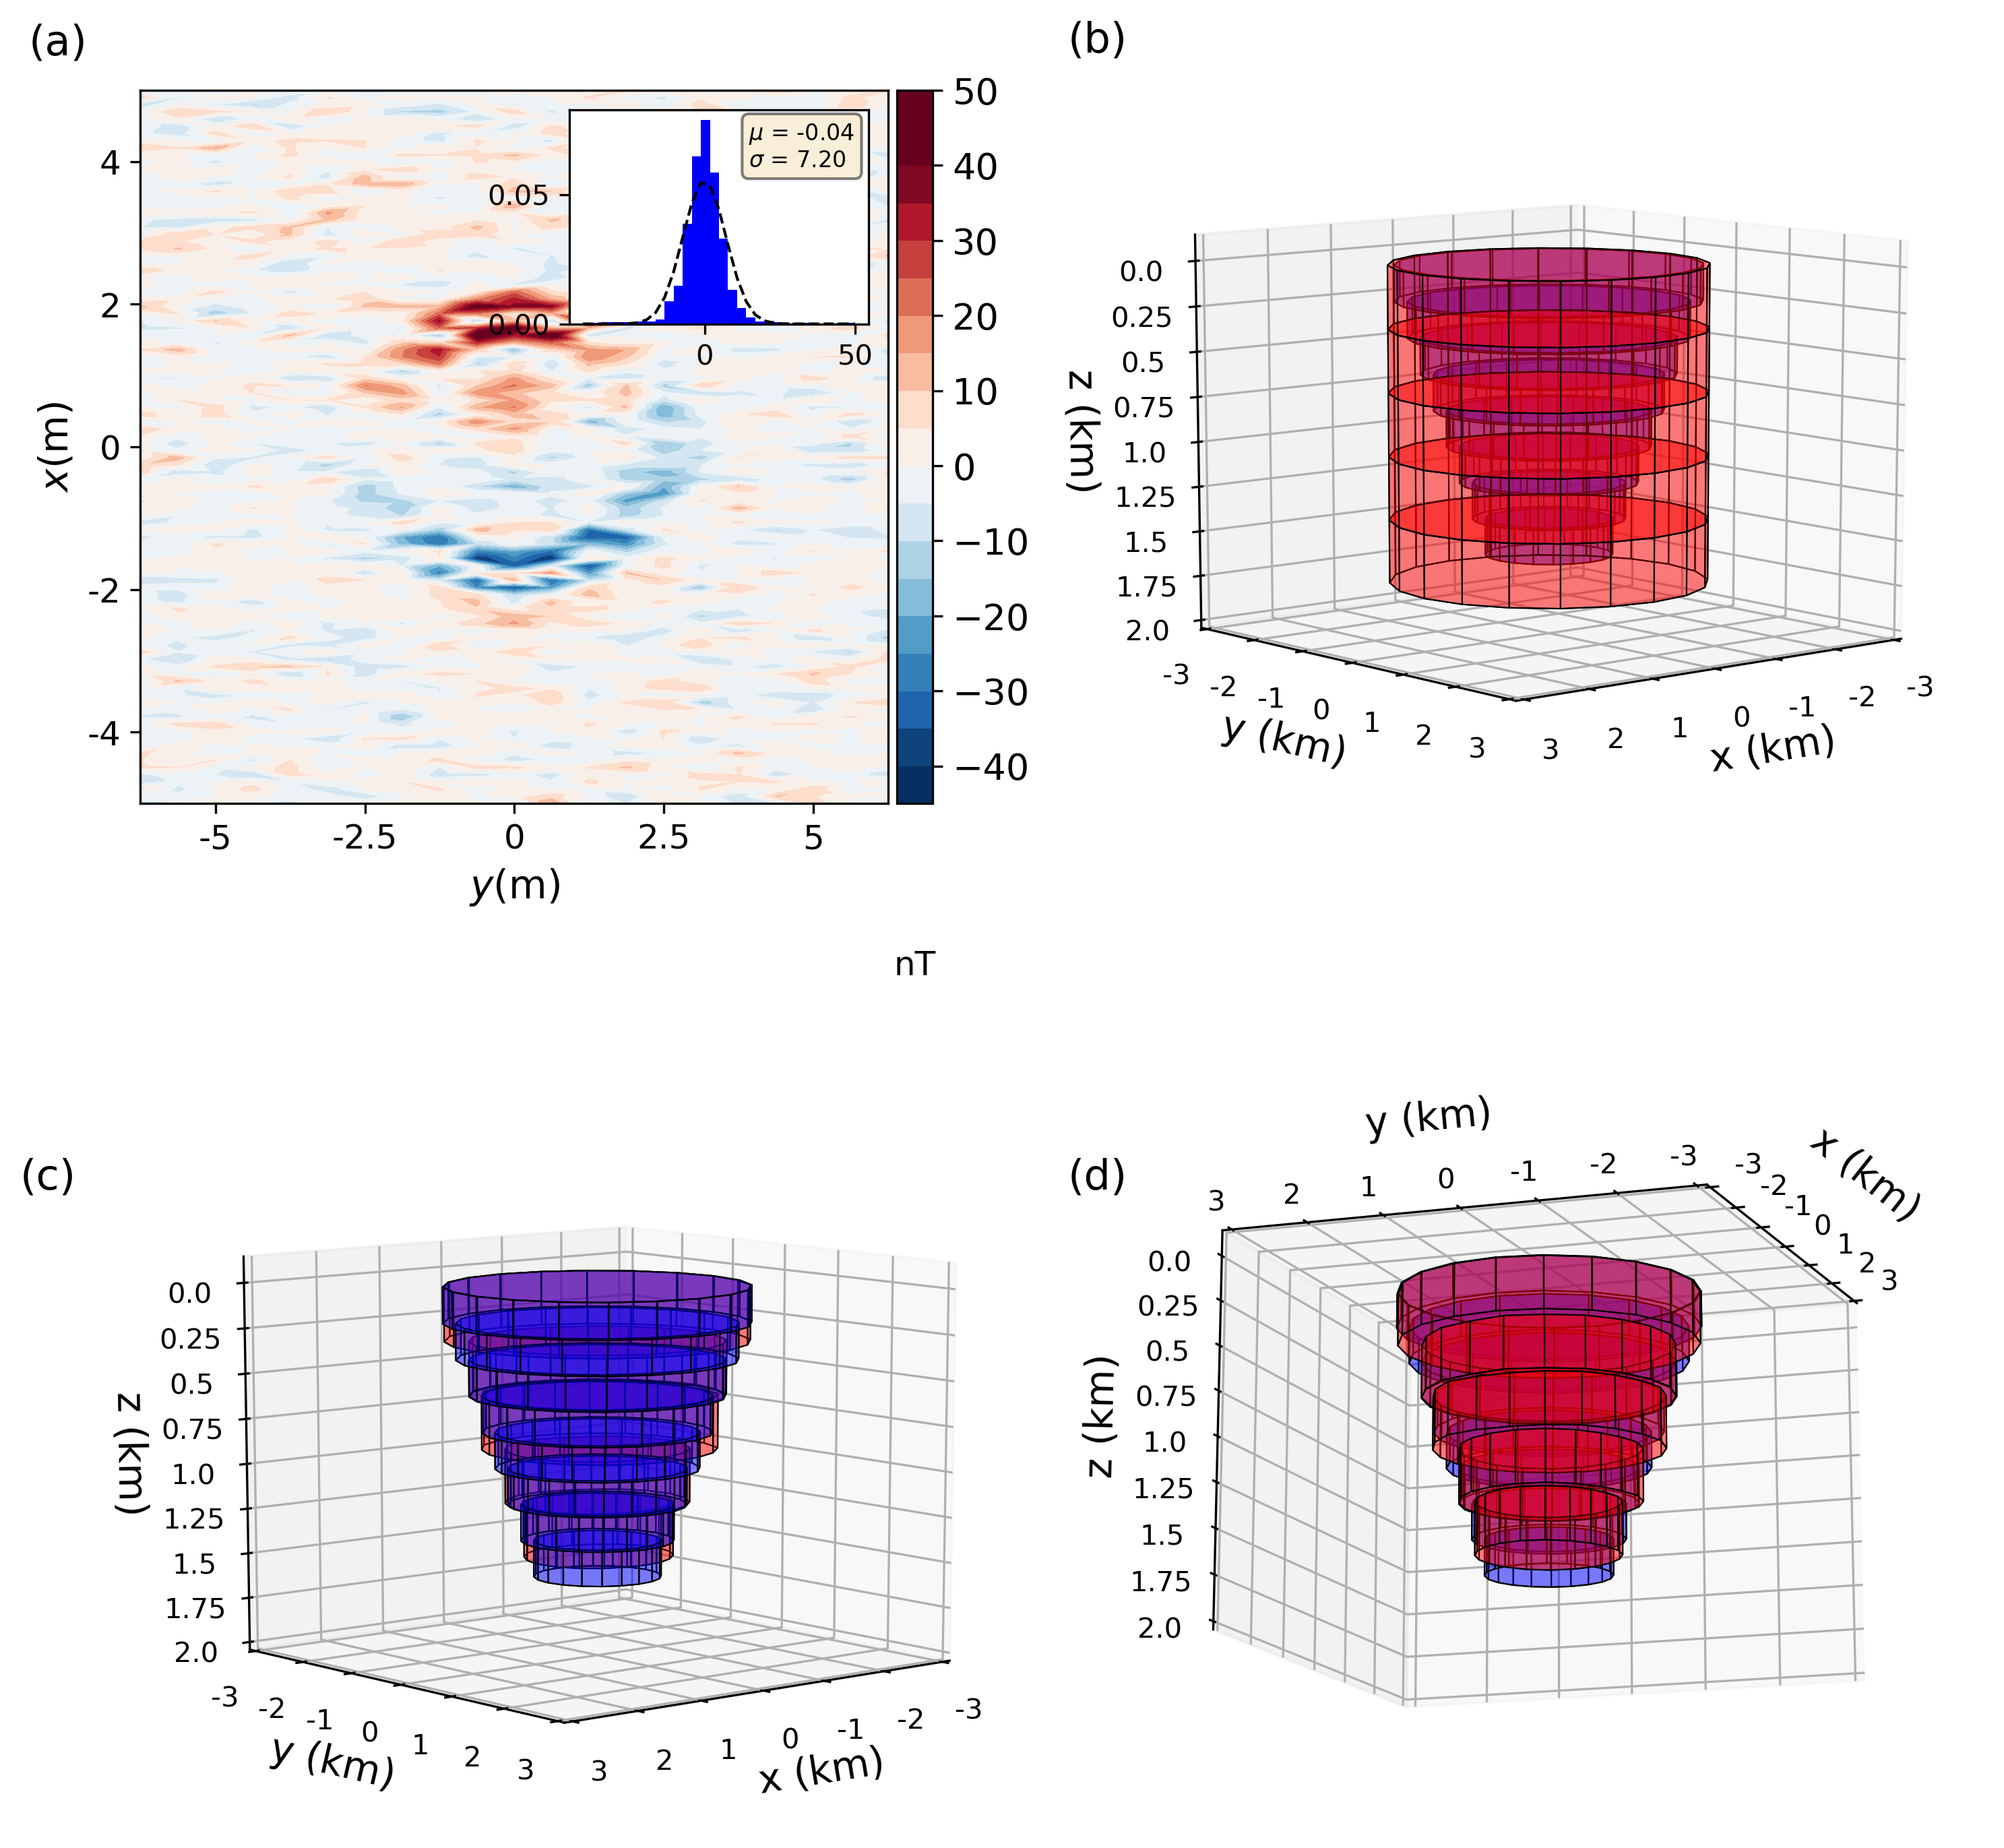
\includegraphics[scale=.5]{figures/simple_results.png}
	\caption{Application to the simple model data. (a) Residuals between the  noise-corrupted data (Fig. \ref{fig:simple_model}a) and the predicted data (not shown) produced by the estimated model. The inset in (a) shows the histogram of the residuals and the Gaussian curve (dashed line) (dashed line) whose mean and standard deviation are, respectively, $\mu = 0.04$ nT and $\sigma=7.20$ nT. (b) Perspective view of the initial approximate (red prisms) and the true model (blue prisms). (c) and (d) Comparison between the estimated source (red prisms) and the true model (blue prisms) in perspective views.}
	\label{fig:simple_results}
\end{figure}

% Application to synthetic data - complex model

\begin{figure}
    \centering
    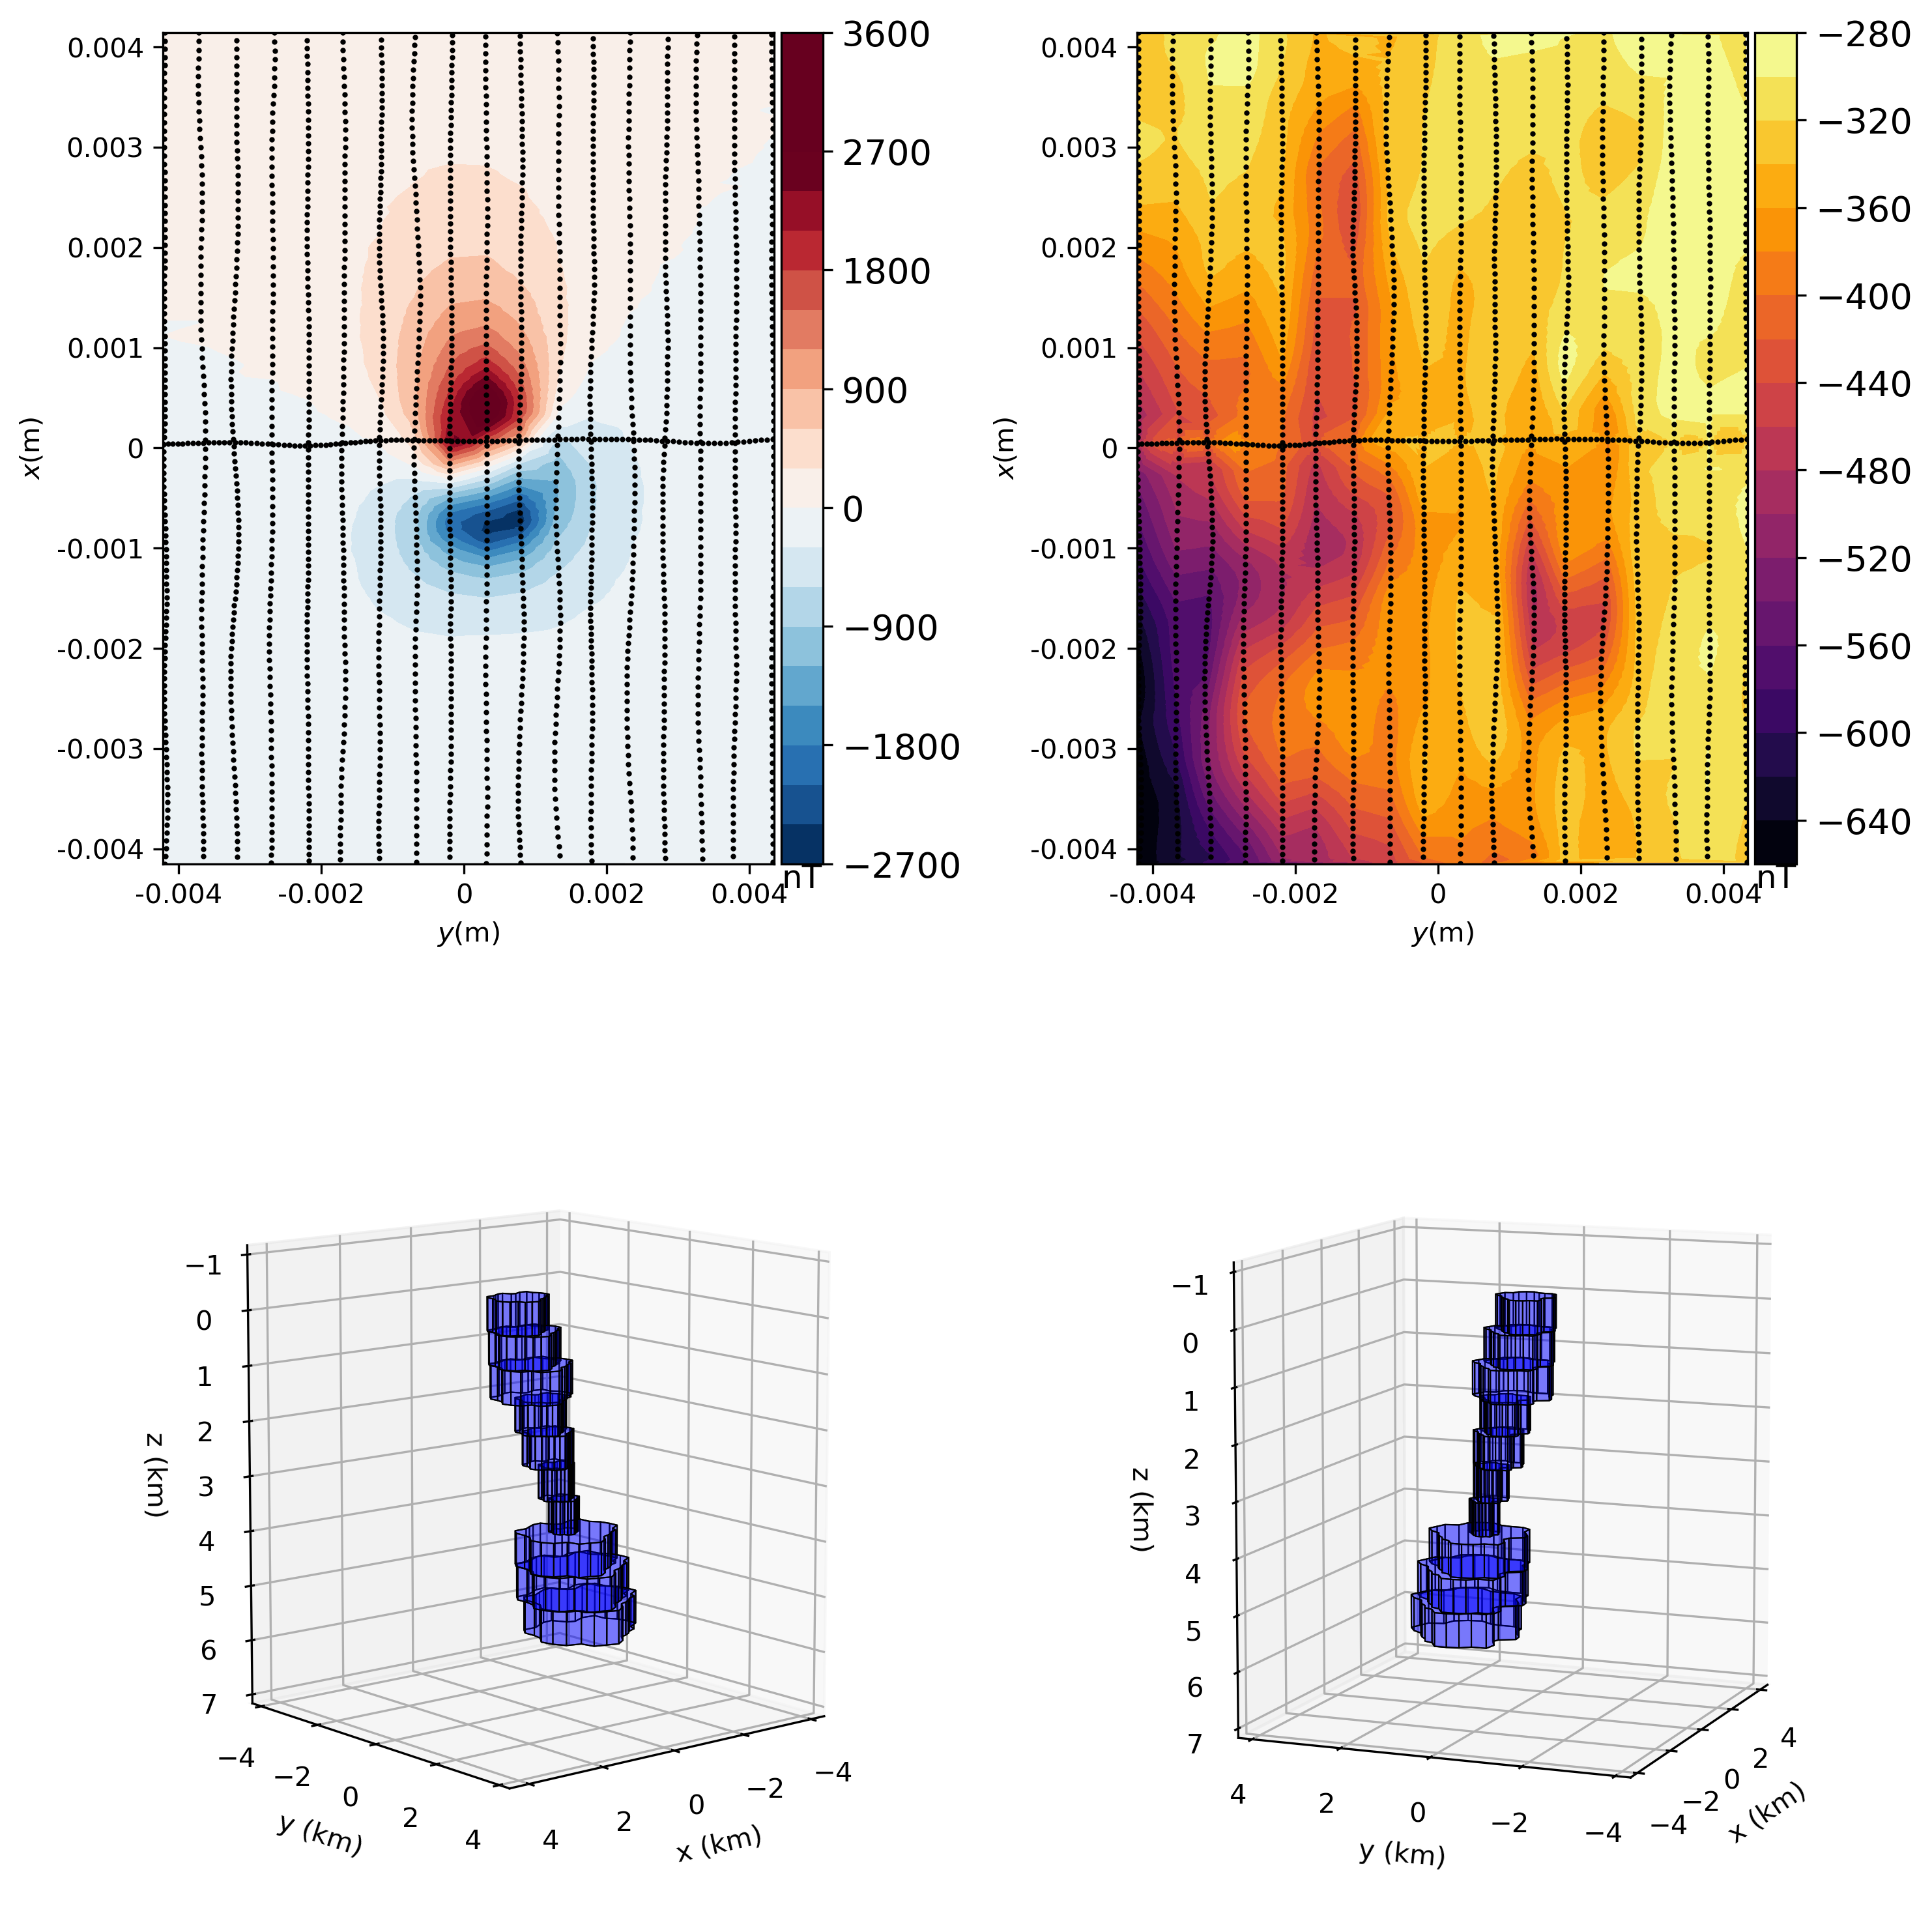
\includegraphics[scale=.5]{figures/complex_model_data.png}
    \caption{Complex model simulation. (a) Noise-corrupted total-field anomaly with a pseudorandom Gaussian distribution having mean $\mu_0 = 0$ nT and standard deviation $\sigma_0 = 5$ nT produced by the complex model, the black dots represent the observation points. The connected red dots are the vertices of the initial approximate horizontally projected at the data map. (b) Vertical coordinates of the observations  simulating an airborne survey. (c) and (d) Perspective views of the complex model represented by the blue prisms.
}
    \label{fig:complex_model}
\end{figure}

\begin{figure}
	\centering
	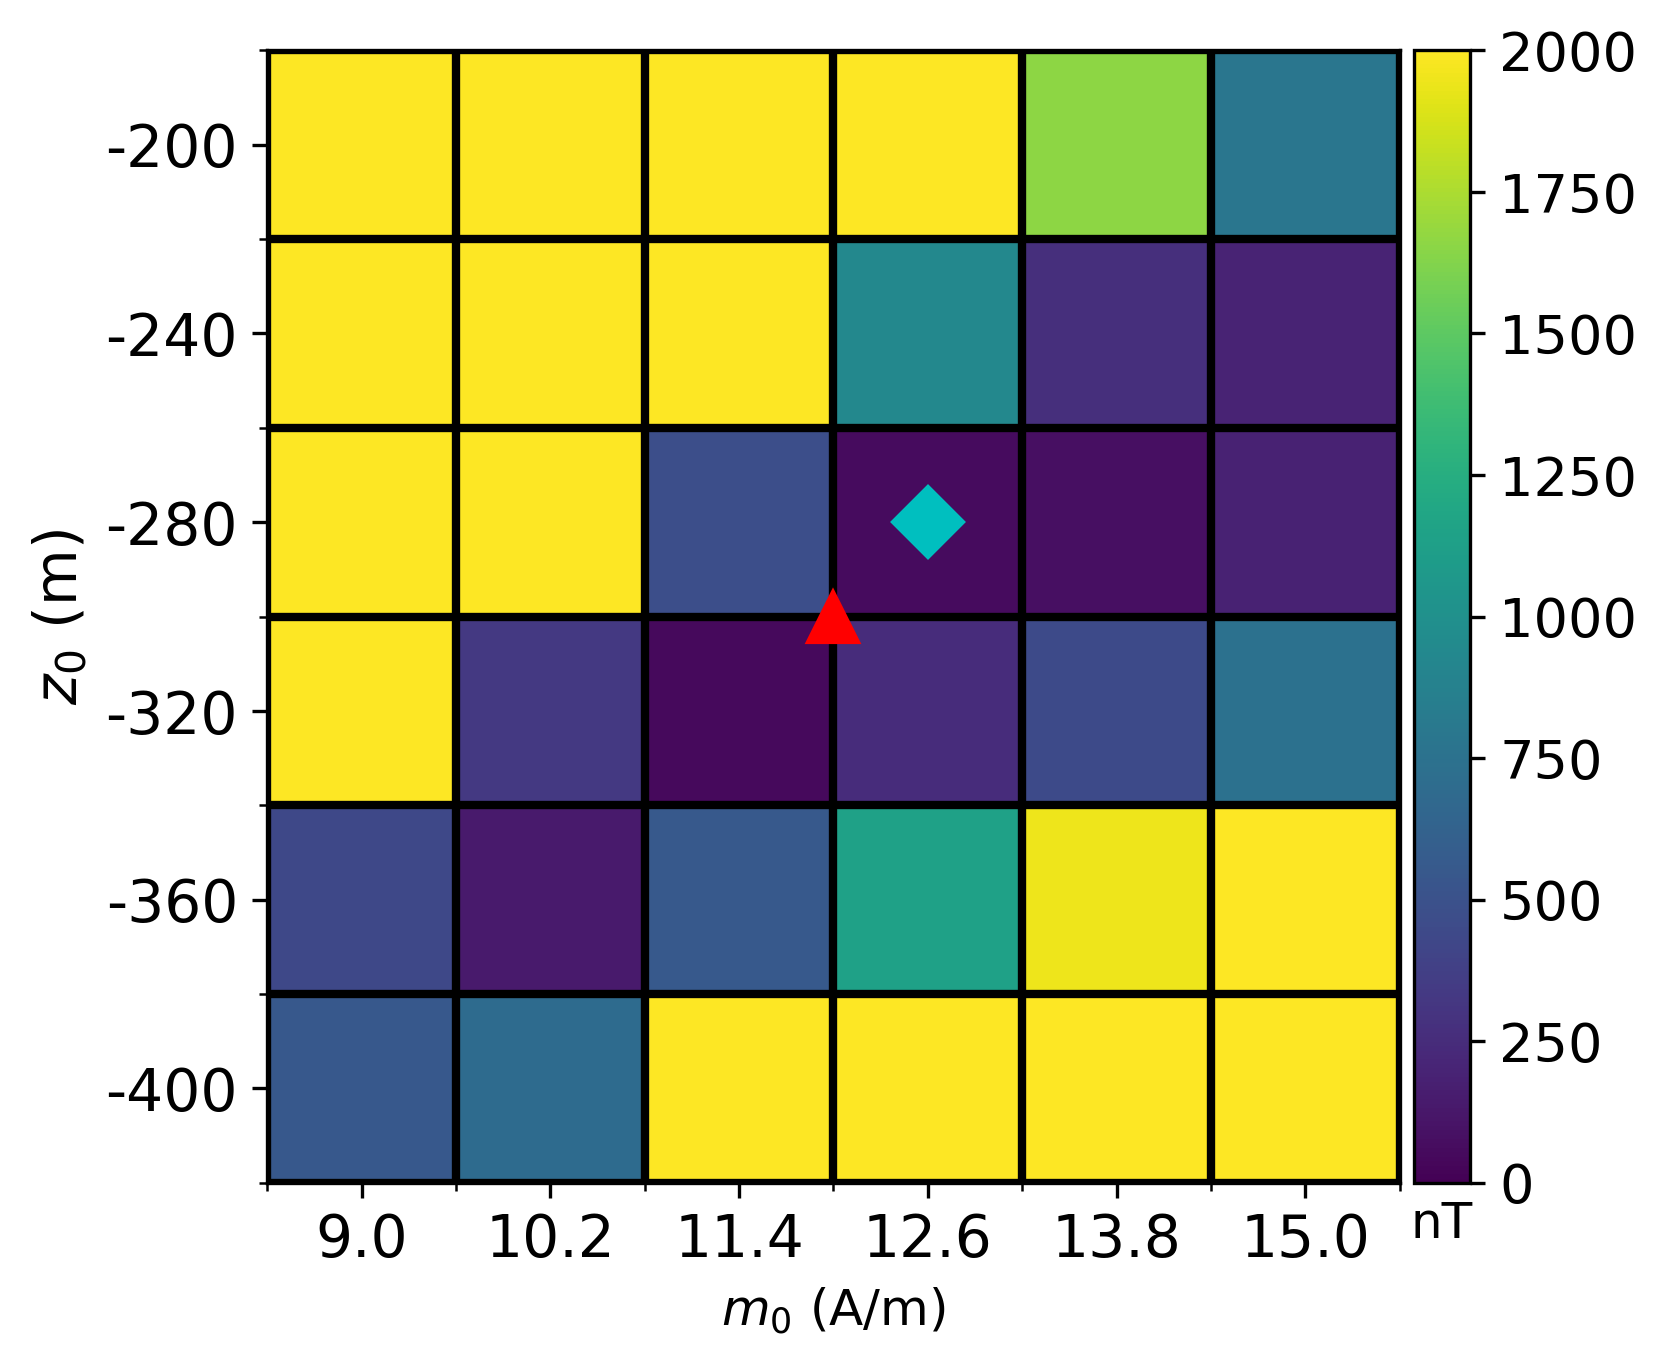
\includegraphics[scale=.75]{figures/complex_gamma.png}
	\caption{Application to the complex model data. 
	Goal function $\Gamma(\mathbf{p})$ (eq. \ref{eq:gamma}), in nT,  
	produced by estimated models with different depths-to-the-top ($ z_0 $) and 
	total-magnetization intensities ($ m_0 $). 
	The red triangle represents the $m_0$ and $z_0$ of the true source. 
	The cyan diamond represents the estimated model that produces the lowest value for $\Gamma (\mathbf{p})$.}
	\label{fig:complex_map}
\end{figure}

\begin{figure}
    \centering
    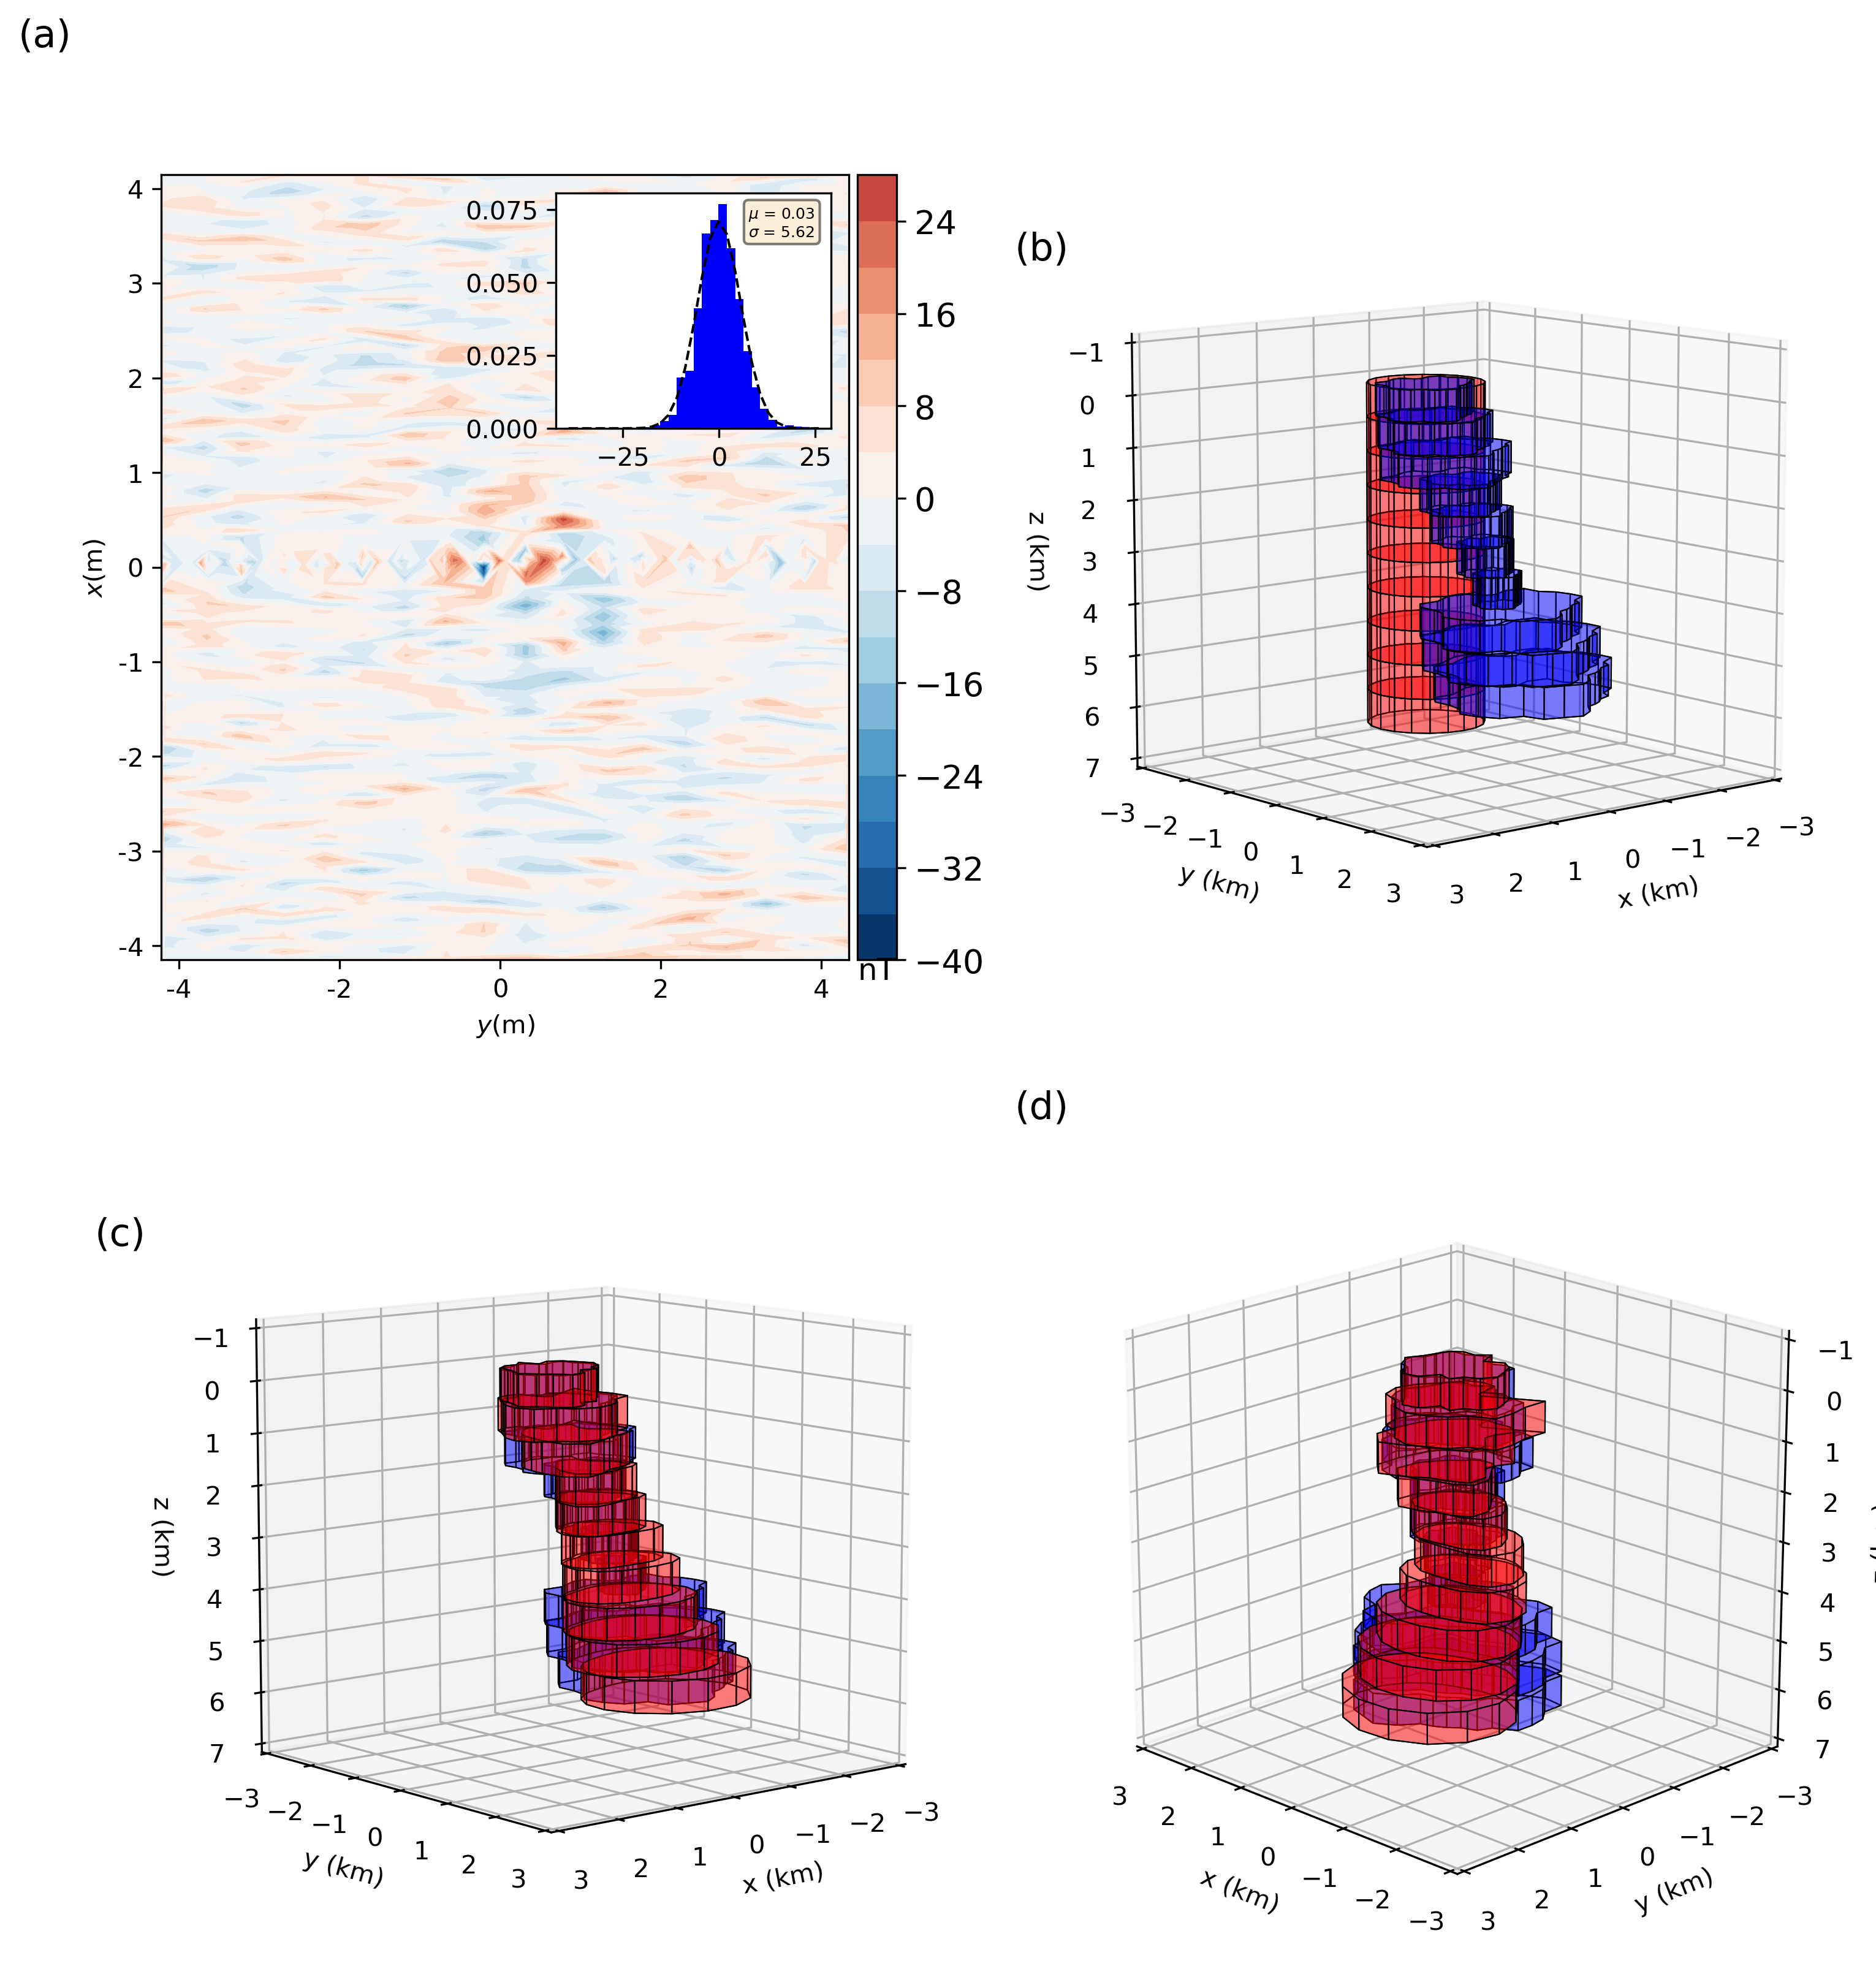
\includegraphics[scale=.5]{figures/complex_results.png}
    \caption{Application to complex model data. (a) Residuals between the noise-corrupted data (Fig. \ref{fig:complex_model}a) and the predicted data (not shown) produced by the estimated model. The inset in (a) shows the histogram of the residuals and the Gaussian curve (dashed line) whose mean and standard deviation are, respectively, $\mu = 0.09$ nT and $\sigma=6.66$ nT. (b) Perspective view of the initial approximate (red prisms) and the true model (blue prisms). (c) and (d) Comparison between the estimated source (red prisms) and the true model (blue prisms) in perspective views. 
}
    \label{fig:complex_result}
\end{figure}

% Application to field data

\begin{figure}
    \centering
    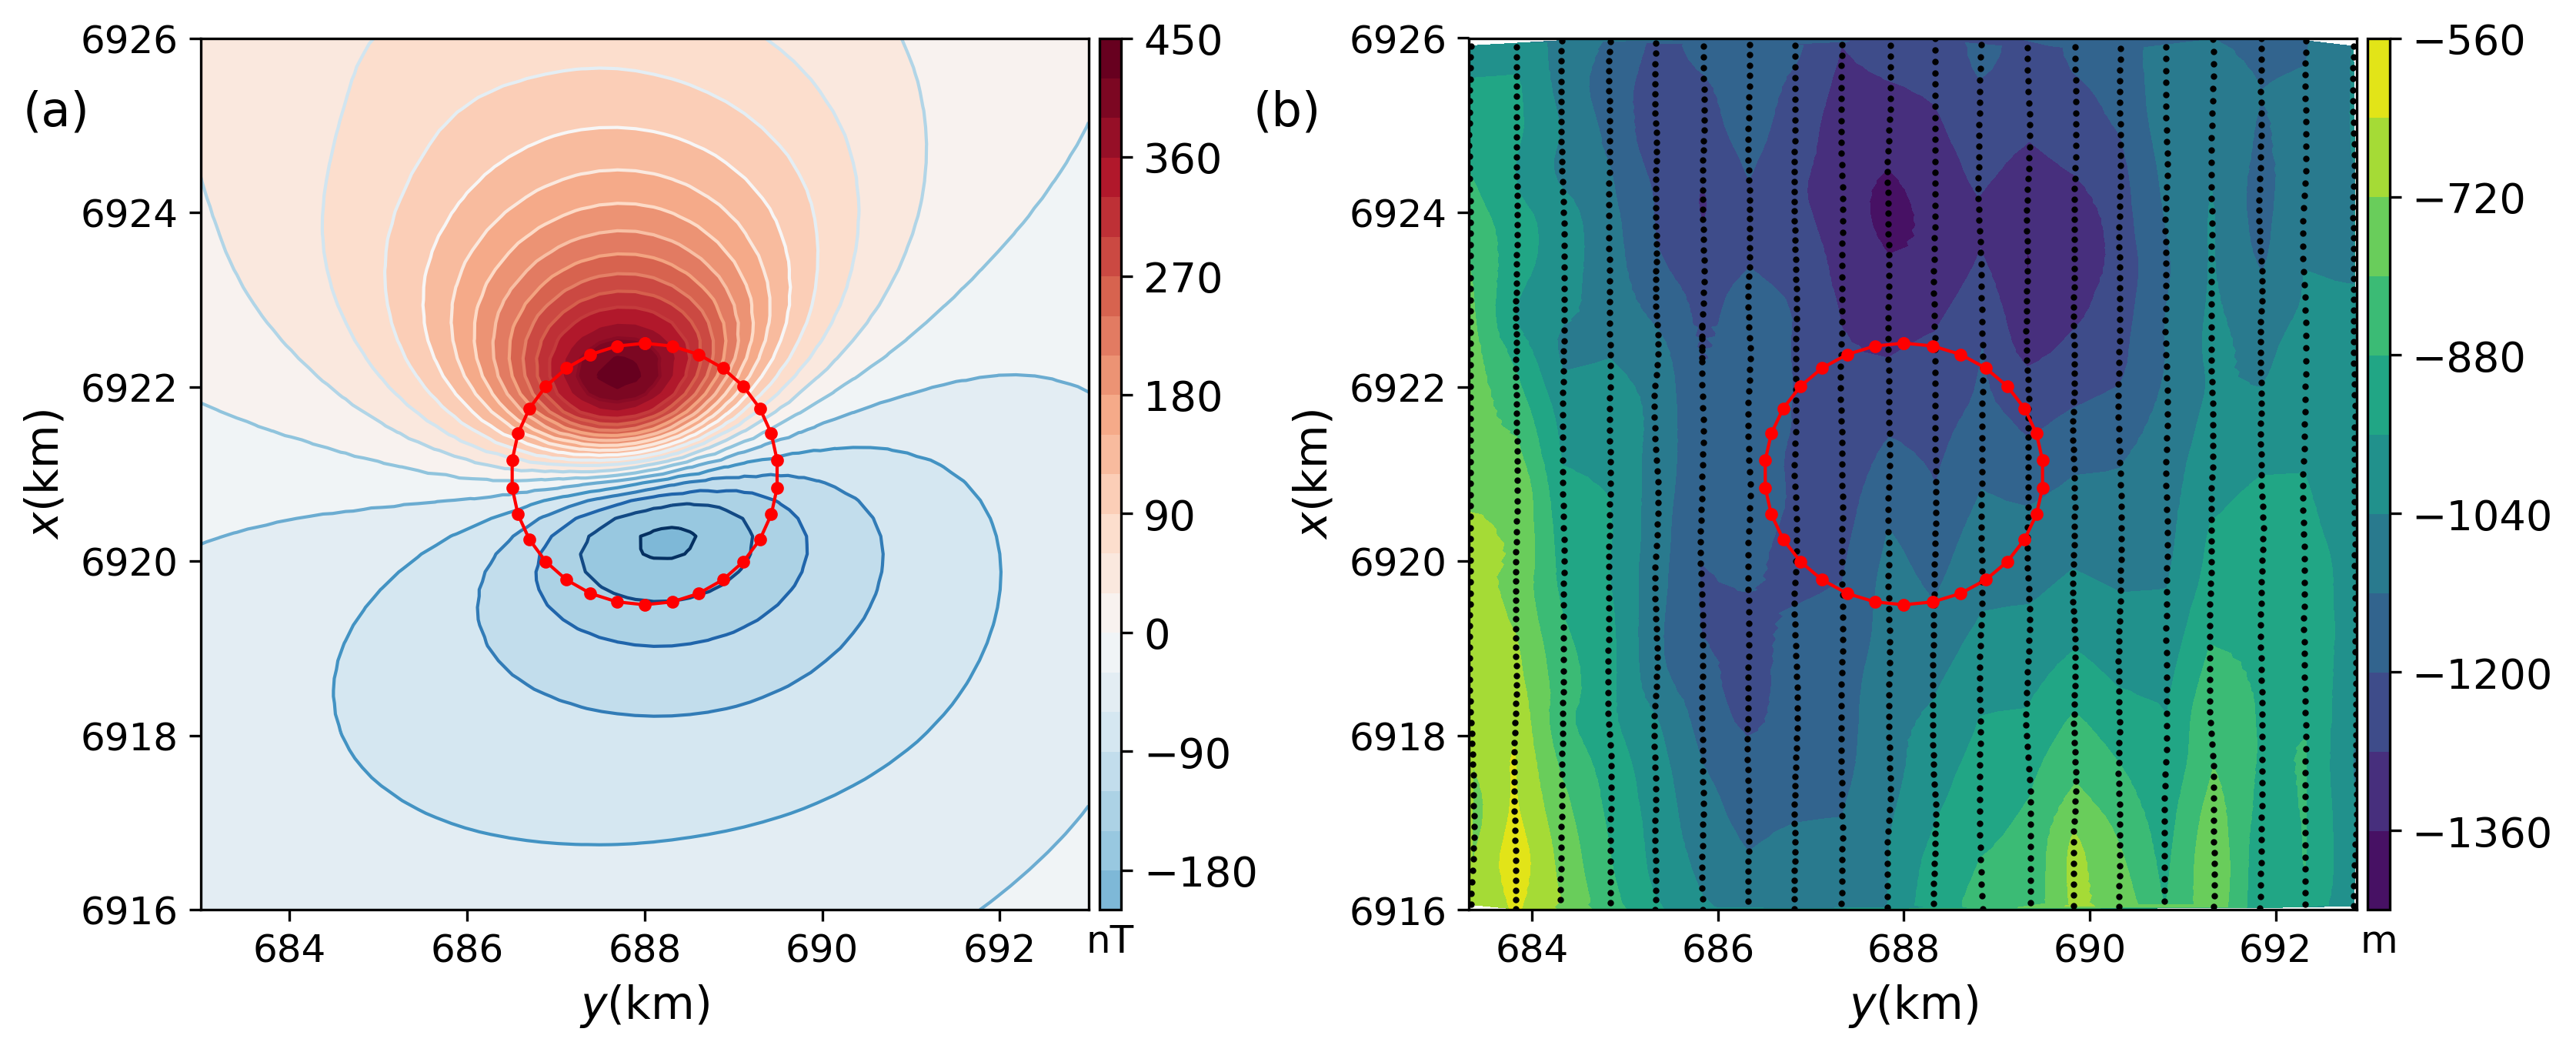
\includegraphics[scale=.5]{figures/real_updata.png}
    \caption{(a) Residual total-field anomaly (in nT) over the  
    Anit{\'a}polis complex, upward-continued to $z = -2000$ m. The horizontal UTM 
    coordinates are referred to the central meridian $ 51^\circ $ W. (b) Geometric 
    height (referred to the WGS84 ellipsoid) of the observation points in m. 
    The black dots are the observation points. The connected red dots in both maps 
    are the projected vertices of the initial approximation $\hat{\mathbf{p}}_{(0)}$ 
    used in the inversion.}
    \label{fig:real_data}
\end{figure}

\begin{figure}
	\centering
	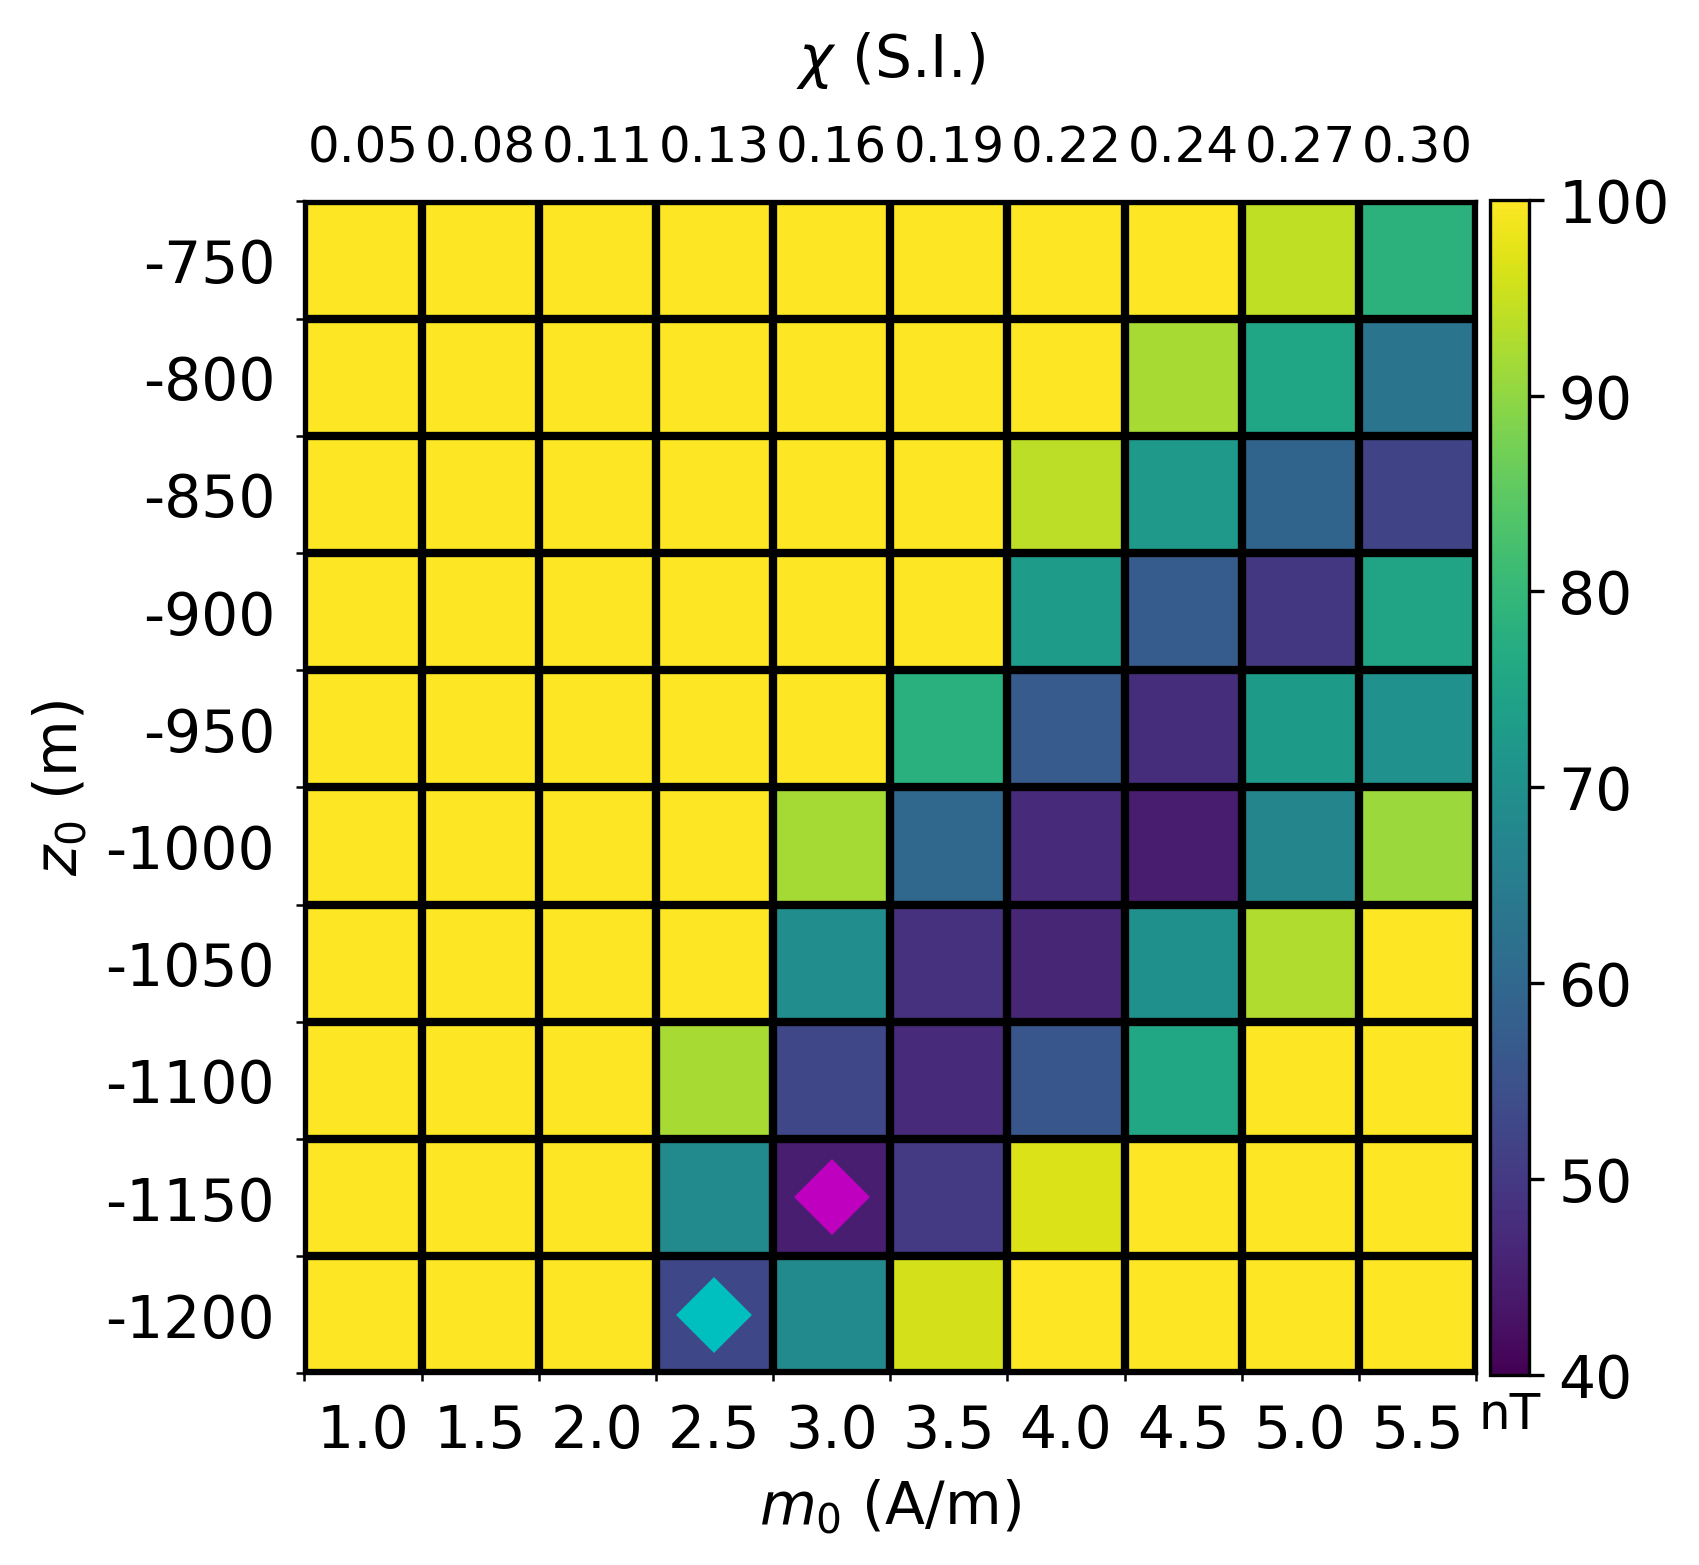
\includegraphics[scale=.75]{figures/real_gamma.png}
	\caption{Application to the field data over the Anit{\'a}polis complex, Brazil. 
	Goal function $\Gamma(\mathbf{p})$ (eq. \ref{eq:gamma}), in nT,  
	produced by estimated models with different depths-to-the-top ($ z_0 $) and 
	total-magnetization intensities ($ m_0 $).
	The corresponding range of magnetic susceptibility $\chi$ is represented in the 
	upper axis by considering a purely induced magnetization with inducing field 
	$\approx 22 \, 768 $ nT.
	The magenta diamond represents the estimated model that produces the lowest value of $ \Gamma(\mathbf{p})$.
	The cyan diamond represents an alternative model whose magnetic susceptibility 
	is also compatible with values found at the Jacupiranga complex in a previous work 
	\citep[][ tb. 1]{valdivia-2009}.}
	\label{fig:real_map}
\end{figure}

\begin{figure}
	\centering
	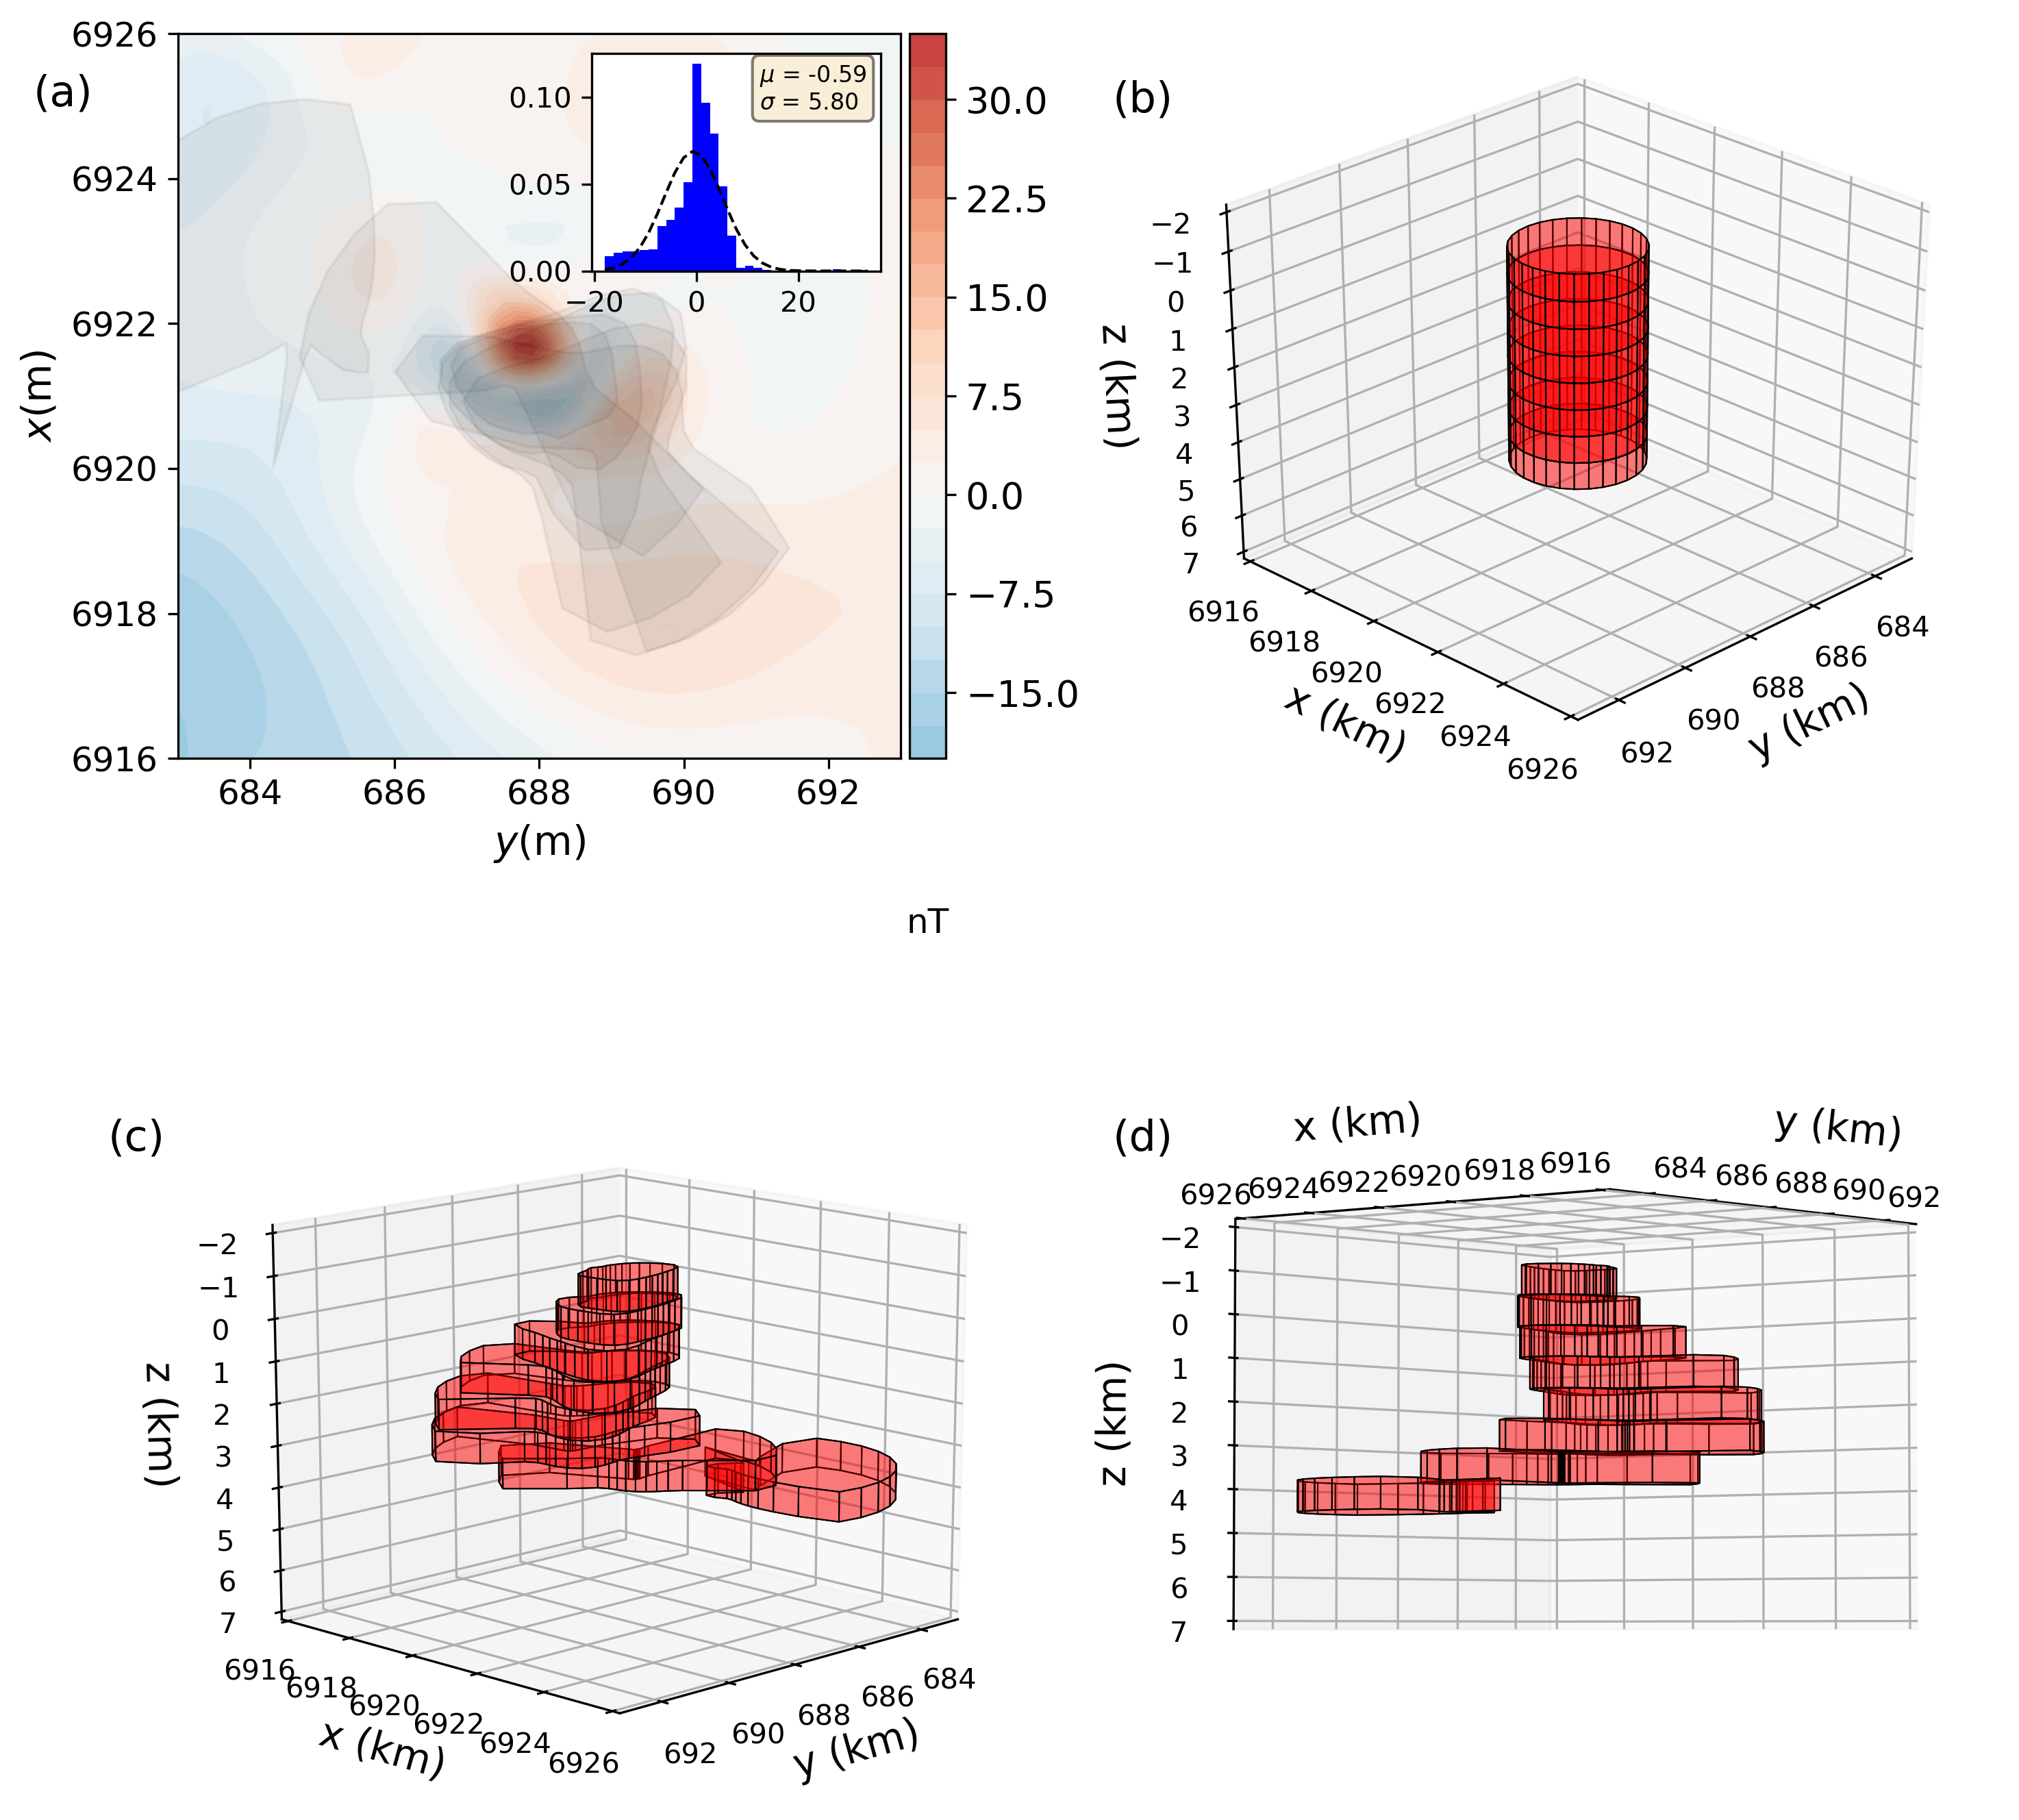
\includegraphics[scale=.5]{figures/real_results_magenta_diamond.png}
	\caption{Application to the field data over the Anit{\'a}polis complex, Brazil.
	Estimated model producing the lowest goal function value, 
	represented by the magenta diamond in Fig. \ref{fig:real_map}.
	(a) Residuals between the observed data (Fig. \ref{fig:real_data}a) and the 
	predicted data (not shown) produced by the estimated model. 
	The inset shows the histogram of the residuals and a normal 
	Gaussian curve (dashed line) with mean and standard deviation 
	$\mu = -0.59$ nT and $\sigma = 5.80$ nT, respectively.
	The light-gray polygons represent the projection of the estimated 
	model on the horizontal plane. 
	(b) Perspective view of the initial approximate (red prisms). 
	(c) and (d) Perspective views of the estimated model (red prisms).}
	\label{fig:real_result2}
\end{figure}

\begin{figure}
    \centering
    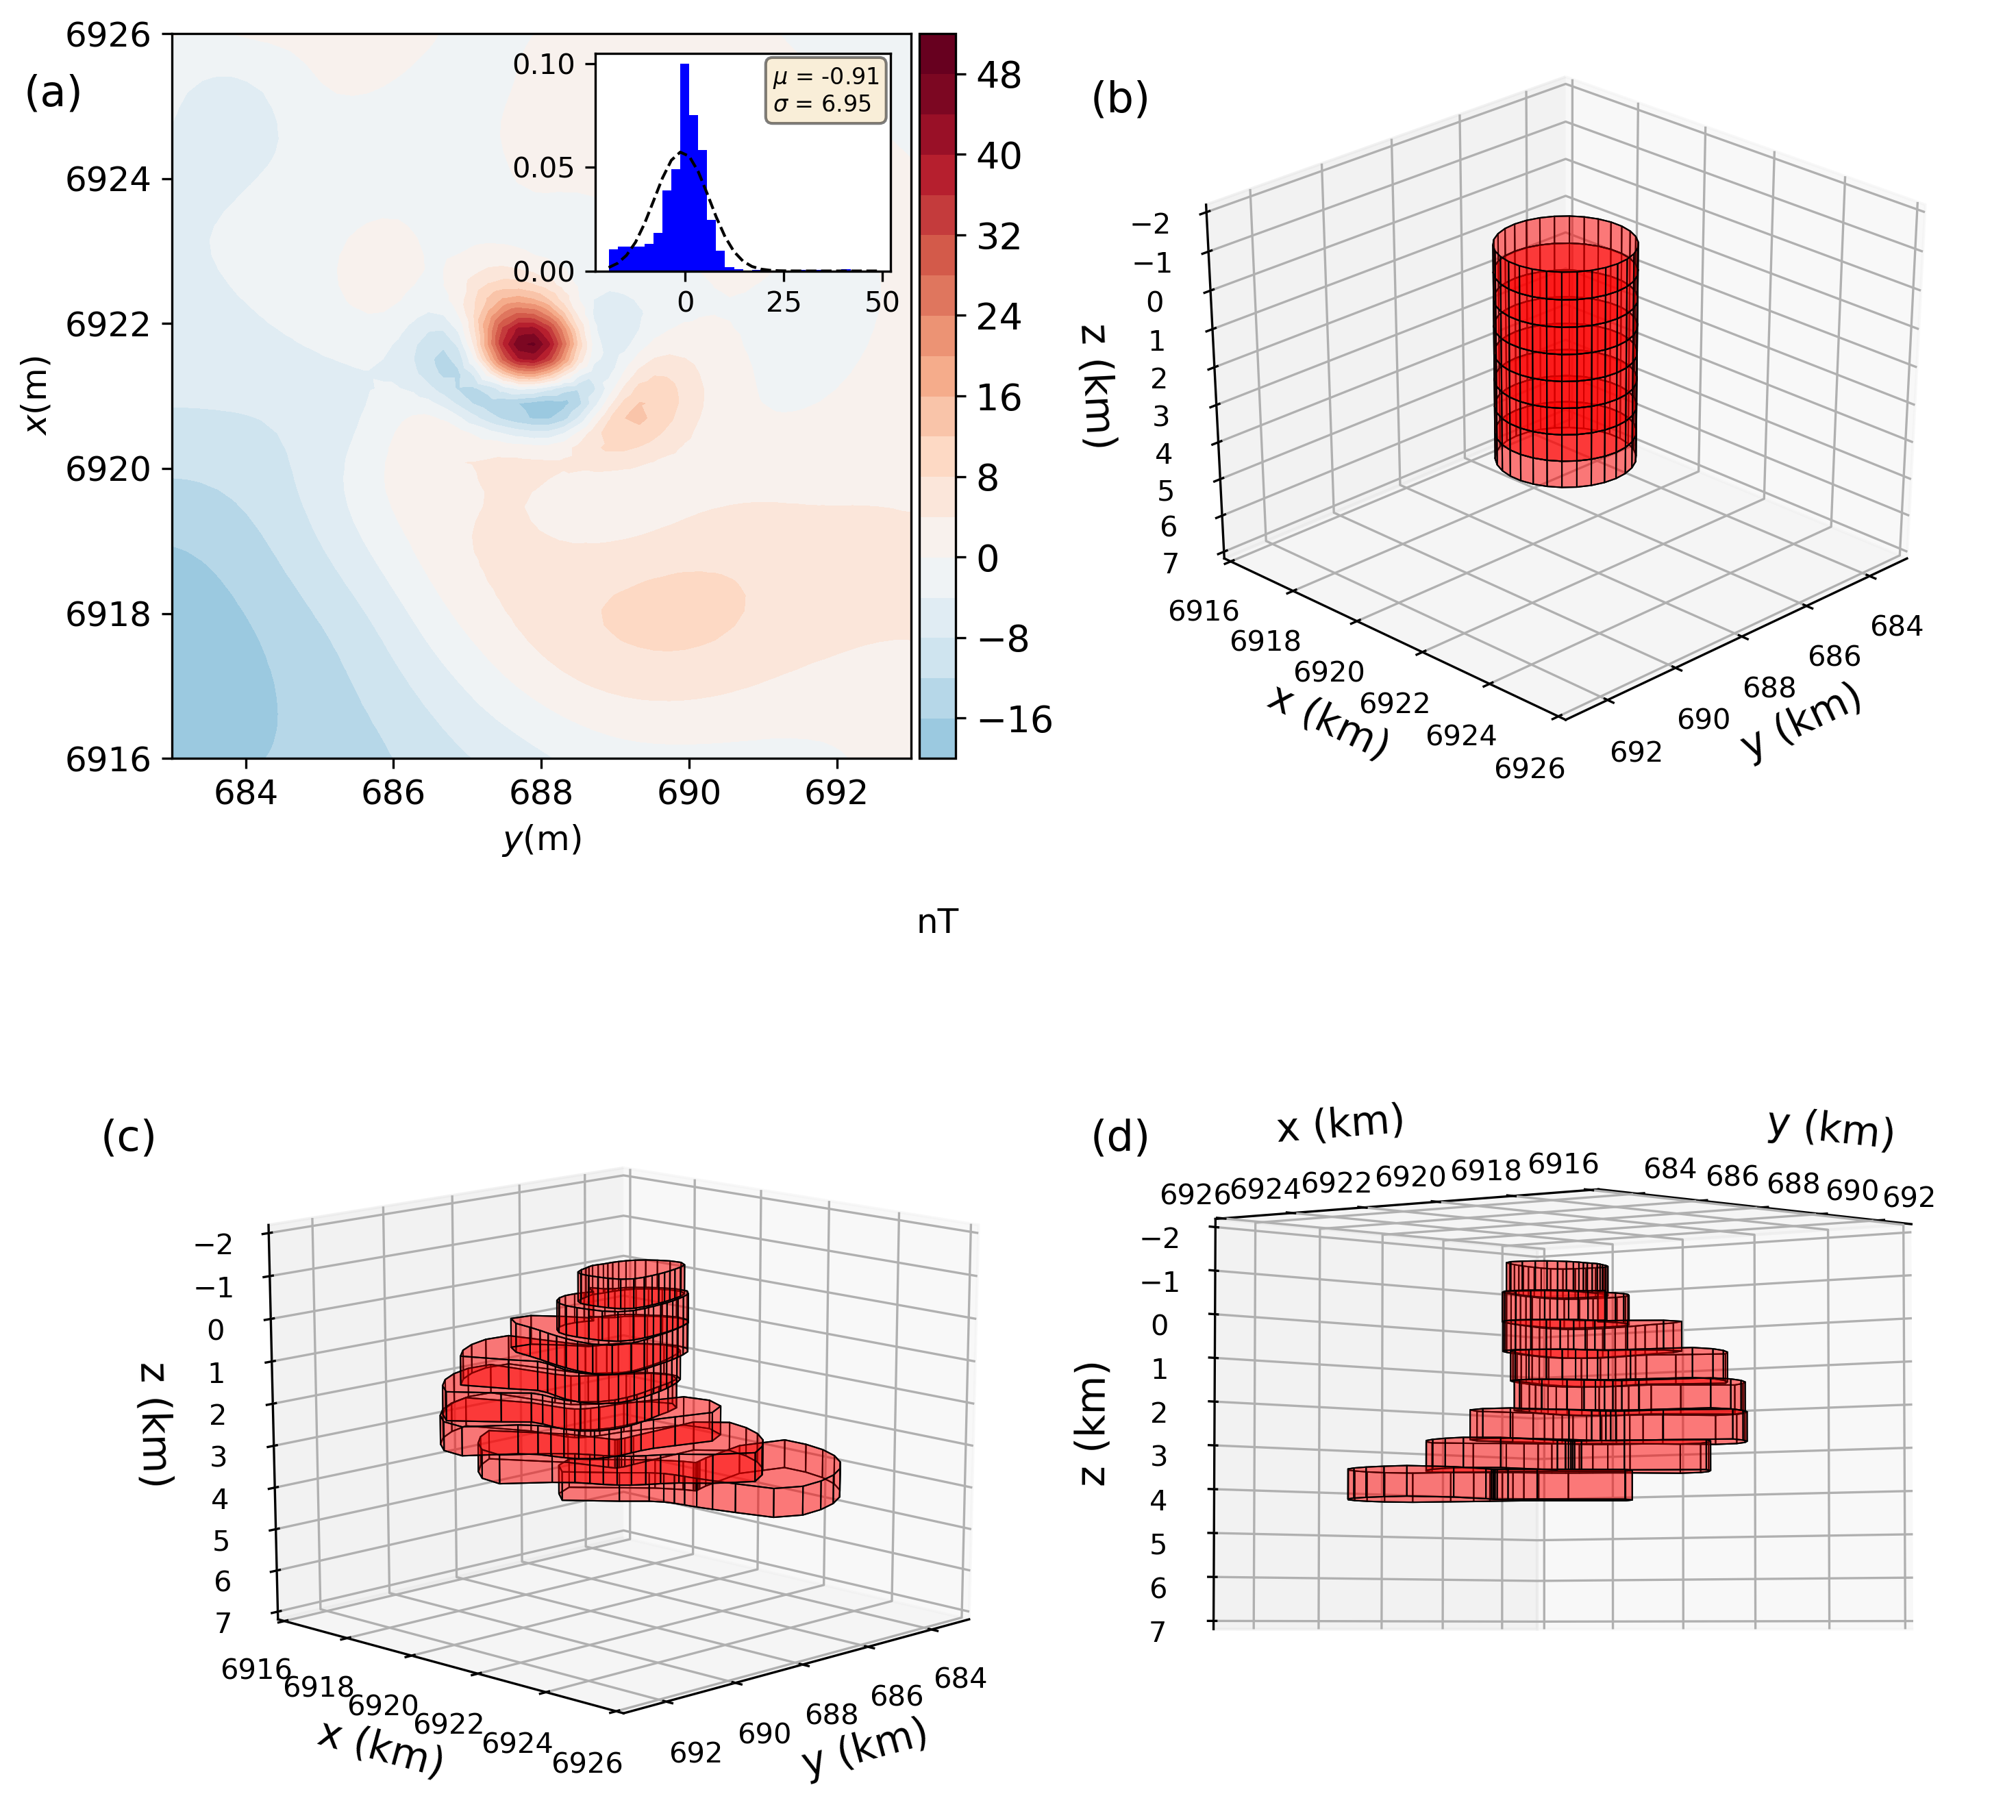
\includegraphics[scale=.5]{figures/real_results_cyan_diamond.png}
    \caption{Application to the field data over the Anit{\'a}polis complex, Brazil.
    Estimated model with magnetic susceptibility value compatible with 
    a priori information close to the study area, 
    represented by the cyan diamond in Fig. \ref{fig:real_map}. 
    (a) Residuals between the observed data (Fig. \ref{fig:real_data}a) and the 
    predicted data (not shown) produced by the estimated model. 
    The inset shows the histogram of the residuals and a normal 
    Gaussian curve (dashed line) with mean and standard deviation 
    $\mu = 0.91$ nT and $\sigma = 6.95$ nT, respectively.
    The light-gray polygons represent the projection of the estimated 
    model on the horizontal plane. 
    (b) Perspective view of the initial approximate (red prisms). 
    (c) and (d) Perspective views of the estimated model (red prisms).}
    \label{fig:real_result}
\end{figure}